\documentclass[aps,floatfix,prd,showpacs]{revtex4}
%\documentclass[aps,floatfix,prd,showpacs,twocolumn]{revtex4}
\usepackage{graphicx}% Include figure files
\usepackage{dcolumn}% Align table columns on decimal point
\usepackage{bm}% bold math

\voffset 1.0cm

\begin{document}

\title{C4.5 CLASSIFICATION ALGORITHM}
\author{
Ameya Keskar                                                         Priya Mane
Chinmay Lotankar                                                     Jeet Mehta
}
\affiliation{
Department of Information Technology
K.J Somaiya College of Engineering,
Mumbai,Maharashtra,
India.}

\date{September 2019}

\begin{abstract}
This article explains the C4.5 algorithm for decision tree construction. C4.5 algorithm works on the principles of Information gain ratio. The comparison between C4.5 and ID3 is also discussed here. Also, the applications of C4.5 algorithm in forming decision trees are explained.  
\end{abstract}


\section{Introduction}

Data mining is the process of analyzing large data and getting valuable information from it. There are various algorithms and techniques done to do so. One such data structure is Decision tree; it is a flowchart-like structure with nodes and arrows directing from one node to another. At each node, one attribute is considered and further split branches equal to the number of unique values the attribute can take. Each of this branch is connected to other node where the value of next attribute is defined. Hence in going from one node to another, we fix or determine the value of each attribute. Each leaf node consists of one of the values of classification variable.
Now the question is which attribute must be placed at what level in a tree.C4.5 Algorithm is used to choose the attributes to be placed at each level of the tree. The main advantage of C4.5 algorithm can deal with attributes having numeric data/non-categorical data which is difficult to classify per say and also deal with missing value data.C4.5 algorithm makes a decision tree by using the concept of information entropy. The parameter used here is normalized information gain. Normalized information gain is calculated for each attribute and the one with maximum value is chosen as the first attribute/root node of the decision tree.


literature review

For the construction of a decision tree, we can use the C4.5 algorithm. The algorithm is based on Information gain entropy. We can say that, if an event is highly probable, there is no surprise if it occurs. This means that it gives very little information. This means amount of information gained is inversely proportional to the probability of the event. Entropy is proportional to the probability of an event; hence we can also say that information gain and entropy are inversely proportional.
In decision trees, it is necessary that with each split the entropy decreases. Hence, if the splitting is done accurately, we may arrive to a very definite decision. So, we check each node for all possible splitting. cases for First, we calculate the entropy difference and the case for which difference is least is considered..

ALGORITHM:
Calculate Information gain for each parameter.
Determine the attribute with maximum Information gain entropy.
Choose this attribute as next splitting node.
Continue in similar manner for all attributes.
 
Let us consider an example 

\begin{figure}
    \centering
    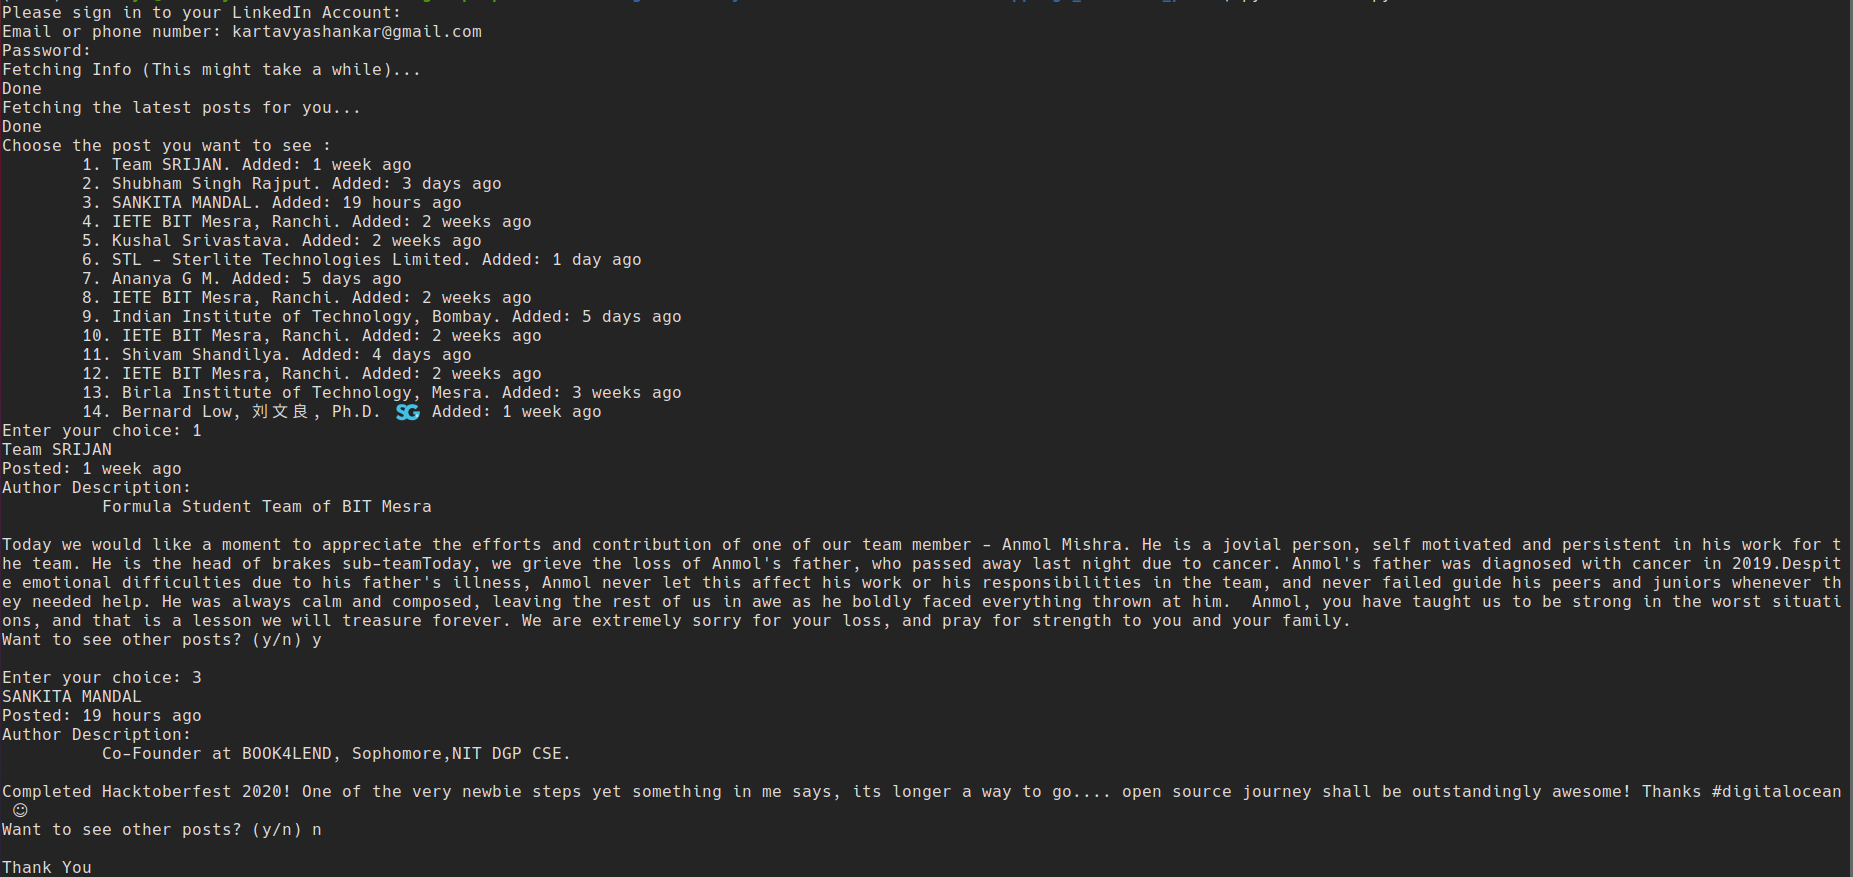
\includegraphics{image1.png}
    \caption{Caption}
    \label{fig:my_label}
\end{figure}

\section{Results}
C4.5 Vs C5.0 C4.5 was superseded in 1997 by a commercial system See5/C5.0 (C5.0 for Unix / Linux, See5 pour Windows).  
The changes hold within new capabilities as well as much improved efficiency, and include: 
  A variant of boosting that constructs an ensemble of classifiers which are then voted to give a final classification. This often leads to a dramatic improvement in predictive accuracy.   New data types (e.g., dates), “not applicable” values, variable misclassification costs, and mechanisms to pre-filter attributes. 
 Unordered rule set when a case is classified, all applicable rules are found and voted. 
 This improves both their predictive accuracy and the interpretability of rule sets.  
Multi-threading enhances scalability. C5.0 have the ability to take advantage of computers with multiple CPUs and/or cores


\section{Conclusions}

The decision tree is a usual algorithm in data mining.C4.5 algorithm is a wide application scope, high frequency decision tree algorithm. It constructs and prunes the decision tree analysis and estimates, completes the classified data mining by data preprocessing and choosing parameters or catalog.The article analyzes the C4.5 and improved methods for the calculation speed of C4.5 algorithm in detail. At least, it is proved by experiment data set that the improved C4.5 algorithm is well-performed on the training speed classify and accuracy. In this Paper C4.5 algorithm was improved the experiment proved that it has minimal impact on the classification accuracy, but the efficiency increased a lot. We can not only speed up the growing of the decision tree, so that better information of rules can be generated. In this paper the algorithm was verified by different large datasets which are publicly available on UCI
machine learning repository. With the improved algorithm ,we can get faster and more effective results without the change of the final decision and the presented algorithm constructs the decision tree more clear and understandable .Efficiency and classification is greatly improved and the disadvantages of low efficiency and memory consumption while dealing with large amount of data were overcome as it was in C4.5.If the amount of data is small original C4.5 is
used because of its higher accuracy.


\acknowledgments
The authors are grateful to K.J Somaiya college of Engineering faculty.

\begin{thebibliography}

https://towardsdatascience.com/what-is-the-c4-5-algorithm-and-how-does-it-work-2b971a9e7db0
https://medium.com/greyatom/decision-trees-a-simple-way-to-visualize-a-decision-dc506a403aeb
https://sefiks.com/2018/05/13/a-step-by-step-c4-5-decision-tree-example/
https://arxiv.org/abs/1310.2071
https://www.sciencedirect.com/science/article/pii/S0925231298000903
https://www.ncbi.nlm.nih.gov/pmc/articles/PMC4466856/



\end{thebibliography}

\end{document}